%\chapter{Related Work}
\section{Fluidic Kernels}
\quad \ \ FluidiCL\cite{FluidicCL}, an OpenCL\cite{OpenCLWeb} runtime that takes a program written for a single device and uses both the CPU and the GPU to execute it. Since they consider a setup with devices having discrete address spaces, their solution ensures that execution of OpenCL work-groups on devices is adjusted by taking into account the overheads for data management. The data transfers and data merging needed to ensure coherence are handled transparently without requiring any effort from the programmer. FluidiCL also does not require prior training or profiling and is completely portable across different machines. Across a set of diverse benchmarks having multiple kernels, our runtime shows a geomean speedup of nearly 64\% over a high-end GPU and 88\% over a 4 core CPU. In all benchmarks, performance of our runtime comes to within 13\% of the best of the two devices.
\begin{figure}[H]
\centering
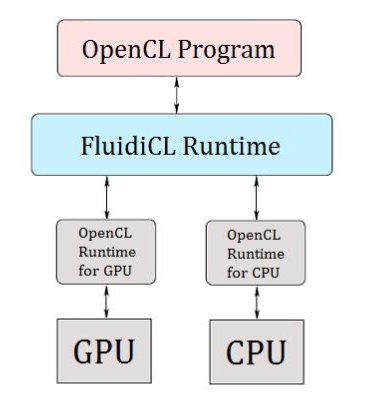
\includegraphics[width=10cm]{img/FluidiCLArch.png}
\caption{Different OpenCL devices and runtimes on FluidiCL}
\label{fig:my_label}
\end{figure}

\begin{figure}[H]
\centering
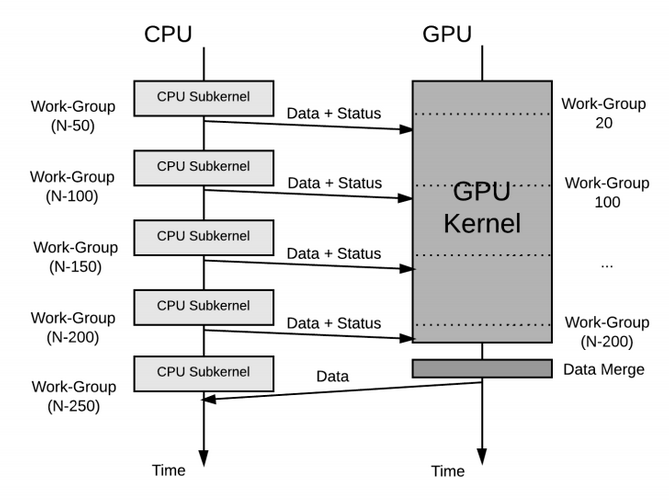
\includegraphics[width=10cm]{img/FluidiCLKernelExecution.png}
\caption{Overview of FluidiCL Kernel Execution}
\label{fig:my_label}
\end{figure}
